\documentclass{article}
\usepackage{tikz}
\usetikzlibrary{trees}
\title{My thirteenth document}
\author{John Doe}
\begin{document}
   \maketitle
   
   The following picture displays a more or less random graph:
   
\begin{figure}[htb]
\center
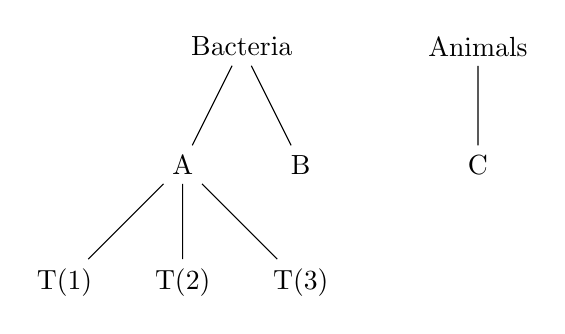
\begin{tikzpicture}[grow=south]
\node (a) {Bacteria} [-]
    child{ node {A}
        child{ node {T(1)} }
        child{ node {T(2)} }
        child{ node {T(3)} }
    }
    child{ node {B} };
\node [right of = a, node distance=3cm] {Animals}
    child{ node {C} };
\end{tikzpicture}
\caption{A simple tree representation}
\label{fig:tree}
\end{figure}

\end{document}
